\documentclass[12pt]{spieman}
\usepackage{amsmath,amsfonts,amssymb}
\usepackage{graphicx}
\usepackage{setspace}
\usepackage{tocloft}
\usepackage[version=4]{mhchem}

% Fix for Unicode characters in bibliography
\usepackage{newunicodechar}
\newunicodechar{κ}{$\kappa$}
\newunicodechar{β}{$\beta$}

\usepackage{lineno}
\linenumbers

% Structured abstract section formatting
\newcommand{\abstractsection}[1]{
  \par\addvspace{.5\baselineskip}
  \noindent\textbf{#1: }\ignorespaces
}

% ---------------------------------------------------------------------------------------
% BEGIN TITLE AND AUTHORS
% ---------------------------------------------------------------------------------------
\title{Visualizing anesthesia-induced vasodilation of cerebral vasculature using multi-exposure speckle imaging}

\author[a]{Colin T. Sullender}
\author[a]{Lisa M. Richards}
\author[b]{Fei He}
\author[b,c]{Lan Luan}
\author[a,*]{Andrew K. Dunn}
\affil[a]{Department of Biomedical Engineering, University of Texas at Austin, 107 W. Dean Keeton Street Stop C0800, Austin, Texas, 78712, United States}
\affil[b]{Department of Electrical and Computer Engineering, Rice University, 6100 Main Street, Houston, TX, 77005, United States}
\affil[c]{Department of Bioengineering, Rice University, 6100 Main Street, Houston, TX, 77005, United States}


% ----------------------------------------------------------------------------------------
% BEGIN DOCUMENT
% ----------------------------------------------------------------------------------------
\renewcommand{\cftdotsep}{\cftnodots}
\cftpagenumbersoff{figure}
\cftpagenumbersoff{table} 
\begin{document} 
\maketitle


% ----------------------------------------------------------------------------------------
% BEGIN ABSTRACT
% ----------------------------------------------------------------------------------------
\begin{abstract}

\abstractsection{Significance}
Anesthetized animal models are used extensively during neurophysiological and behavioral studies despite systemic effects from anesthesia that undermine both accurate interpretation and translation to awake human physiology. The majority of work examining the impact of anesthesia on cerebral blood flow (CBF) has been limited to before and after measurements with limited spatial resolution.

\abstractsection{Aim}
Characterize the effects of isoflurane on CBF during the induction of general anesthesia using multi-exposure speckle imaging (MESI).

\abstractsection{Approach}
Head-restrained awake mice were continuously imaged with MESI as general anesthesia was induced with isoflurane. MESI was used to estimate changes in cortical hemodynamics including vessel size, vascular flow, and parenchyma perfusion across multiple imaging sessions and animals. 

\abstractsection{Results}
The large anatomical changes caused by isoflurane are depicted with wide-field imagery and video highlighting the induction of anesthesia. Compared to the awake state, we measured, on average, an 18\% increase in surface vessel diameter accompanied by a 135\% increase in vascular flux and 92\% increase in parenchyma perfusion.

\abstractsection{Conclusions}
The large alterations caused by isoflurane anesthesia to the cortical vasculature and CBF are unrepresentative of normal physiology and provide further evidence that neuroscience experiments would benefit from transitioning to un-anesthetized awake animal models.

\end{abstract}

% Include a list of up to six keywords after the abstract
\keywords{multi-exposure speckle imaging, laser speckle contrast imaging, awake imaging, anesthesia, isoflurane, cerebral blood flow}

% Include email contact information for corresponding author
{\noindent \footnotesize\textbf{*}Andrew K. Dunn, \linkable{adunn@utexas.edu}}

\begin{spacing}{2}   % use double spacing for rest of manuscript


% ----------------------------------------------------------------------------------------
% BEGIN INTRODUCTION SECTION
% ----------------------------------------------------------------------------------------
\section{Introduction}
\label{sect:introduction}

The use of general anesthesia during neuroimaging is ubiquitous across many animal models despite systemic effects on neurophysiological state and cardiovascular function \cite{Slupe:2018ea}. Volatile inhalation anesthetics, such as the halogenated ether isoflurane \cite{Eger:1981ia}, are commonly utilized to immobilize animals during imaging while allowing for fine control over the depth of anesthesia and consciousness. However, isoflurane has been shown to reduce neuronal activity \cite{Aksenov:2015ea} and functional connectivity \cite{Xie:2019de}, suppress the magnitude and speed of neurovascular coupling \cite{Masamoto:2012bj,Takuwa:2012ee,Pisauro:2013cx}, and induce significant vasodilation \cite{Koenig:1994rn,Strebel:1995uh,Iida:1998th}. Isoflurane also conveys potential neuroprotective effects that reduce and delay the severity of cerebral ischemia \cite{Kitano:2007ia,Kawaguchi:2000id,Sakai:2007wc,Li:2013ip,Lu:2017bo}. These effects can mask the benefits of prospective neuroprotective therapeutics or interventions and confound the outcomes of long-term studies \cite{Kapinya:2002ua,Seto:2014ga}. For these reasons and more \cite{Gao:2017tw}, there is a growing effort within the neuroscience community to transition to un-anesthetized awake animal models in order to more accurately interpret neurophysiological and behavioral experiments and more readily translate findings to awake human physiology.

There have been numerous imaging modalities used to examine the effects of isoflurane on cerebral hemodynamics. Functional magnetic resonance imaging (fMRI), laser Doppler flowmetry, and intrinsic signal optical imaging have all established that isoflurane increases basal cerebral blood flow (CBF) while attenuating and delaying the hemodynamic response to local neural activity via neurovascular coupling \cite{Sicard:2003dj,Desai:2011mb,Aksenov:2015ea,Takuwa:2012ee,Pisauro:2013cx}. Two-photon phosphorescence lifetime microscopy showed that tissue oxygenation is twice as high under isoflurane anesthesia compared to the awake state and exhibited large layer-specific differences within the cortical vasculature \cite{Lyons:2016bd}. Calcium signal imaging following ischemic stroke found that the magnitude of spreading depolarizations were significantly smaller in awake mice \cite{Balbi:2017cj} while laser speckle contrast imaging (LSCI) of photothrombotic stroke observed larger infarct sizes in awake rats compared to their isoflurane-anesthetized counterparts \cite{Lu:2017bo}. To our knowledge, no prior studies have directly monitored the induction of general anesthesia and its acute effects upon the cerebral vasculature.

In this paper, we present multi-exposure speckle imaging (MESI) of cerebral blood flow in awake mice during the induction of general anesthesia with isoflurane. The MESI technique \cite{Parthasarathy:2008el} provides a more robust estimate of large changes in flow compared to traditional single-exposure LSCI \cite{Parthasarathy:2010vo} and enables the chronic tracking of CBF \cite{Kazmi:2013hp}. We highlight the large anatomical and physiological changes to cortical hemodynamics in response to isoflurane with wide-field imagery across multiple imaging sessions and animals. Because the anesthetized state is representative of an abnormal physiology, we argue that awake animal models should be utilized whenever possible for neuroscience studies.


% ----------------------------------------------------------------------------------------
% BEGIN METHODS SECTION
% ----------------------------------------------------------------------------------------
\section{Methods}
\label{sect:methods}

\subsection{Multi-Exposure Speckle Imaging (MESI)}
A schematic of the imaging system is presented in Fig.~\ref{fig:system_image}a. MESI was performed using a 685 nm laser diode (50 mW, HL6750MG, Thorlabs, Inc.) intensity modulated with an acousto-optic modulator (AOM, 3100-125, Gooch \& Housego, Ltd.) and relayed to illuminate the craniotomy at an oblique angle. The scattered light was imaged by a CMOS camera (acA1920-155um, Basler AG) with $2\times$ magnification and cropped to a field-of-view of 3.6 $\times$ 3.0 mm. Camera exposures were temporally synchronized with the modulated laser pulses. Fifteen camera exposures ranging between 50 $\mu$s and 80 ms \cite{Parthasarathy:2008el,Atchia:2013ep,Kazmi:2013hp} were recorded for each complete MESI frame in order to broadly sample the speckle dynamics of the specimen \cite{Kazmi:2014go}, resulting in an effective acquisition rate of $\sim$2.5 MESI frames-per-second. The total amount of light used to capture each exposure was held constant with the AOM in order to minimize the effects of shot noise \cite{Parthasarathy:2008el}. The acquisition was controlled using custom software written in C++ along with a multifunction I/O device (USB-6363, National Instruments Corp.) for the generation of camera exposure trigger signals and AOM modulation voltages \cite{Sullender:2018ff}.

The 15 raw intensity images were converted to speckle contrast images ($K = \sigma_{s} / {\langle{I}\rangle}$) with a 7$\times$7-pixel sliding window and used to calculate an estimate of the speckle correlation time ($\tau_c$) at each pixel with the multi-exposure speckle visibility expression \cite{Parthasarathy:2008el}:
%
% Equation 1 - MESI Equation
\begin{equation}
    \label{eq:mesi}
    K(T,\tau_c) =
        \left(
        \beta\rho^2\frac{e^{-2x} - 1 + 2x}{2x^2} +
        4\beta\rho(1 - \rho)\frac{e^{-x} - 1 + x}{x^2} +
        \beta(1 - \rho)^2 +
        \nu_{noise}
        \right)^{1/2}
\end{equation}

\noindent where $T$ is the camera exposure time, $x = T/\tau_c$, $\rho$ is the fraction of light that is dynamically scattered, $\beta$ is a normalization factor that accounts for speckle sampling, and $\nu_{noise}$ represents exposure-independent instrument noise and nonergodic variances. Eq.~(\ref{eq:mesi}) was fitted with the Levenberg-Marquardt nonlinear least squares algorithm \cite{Lourakis:2005} using a custom program written in C.

Because $\tau_c$ is inversely related to the speed of the moving scatterers \cite{Bonner:1981hg,Briers:1996kfa}, the inverse correlation time ($ICT = 1/\tau_c$) is frequently used as a metric for quantifying blood flow in vasculature and perfusion in parenchyma \cite{Ayata:2004ba,Strong:2005kj,Sullender:2018ff}. Recent work to improve the quantitative accuracy of MESI flow measurements in vasculature takes into account the presence of multiple dynamic scattering events instead of assuming only a single dynamic scattering event per photon \cite{Kazmi:2015du}. This is achieved by scaling the fitted $ICT$ value by the diameter of the vessel in order to obtain an estimate of ``vascular flux'' that better accounts for variations in vascular volume sampling \cite{Kazmi:2015du,Richards:2017df}. This paper uses the vascular flux metric (arbitrary units) for all vessel measurements and $ICT$ (s$^{-1}$) for all parenchymal perfusion measurements.


% ----------------------------------------------------------------------------------------

\subsection{Animal Preparation}

Mice ($n = 4$, C57BL/6J, male, 4-6 months, Charles River Laboratories, Inc.) were anesthetized with medical \ce{O2} vaporized isoflurane (3\% for induction, 1-2\% for maintenance, 0.5 L/min) via nose-cone inhalation. Body temperature was maintained at 37 $^\circ$C with a feedback heating pad (DC Temperature Controller, Future Health Concepts, Inc.). Arterial oxygen saturation, heart rate, and breathing rate were monitored via pulse oximetry (MouseSTAT, Kent Scientific Corp.). Mice were placed supine in a stereotaxic frame (Kent Scientific Corp.) and subcutaneously administered carprofen (5 mg/kg) and dexamethasone (2 mg/kg) to reduce inflammation during the craniotomy procedure. The scalp was shaved and resected to expose the skull between the bregma and lambda cranial coordinates. A circular region (4 mm diameter) of the skull including the dura mater over the somatosensory cortex was removed with a dental drill (Ideal Microdrill, 0.8 mm burr, Fine Science Tools, Inc.) while under regular artificial cerebrospinal fluid (buffered pH 7.4) perfusion. A 4 mm round \#1.5 cover glass (World Precision Instruments, Inc.) was placed over the exposed brain with artificial cerebrospinal fluid filling the void. Gentle pressure was applied to the cover glass while Kwik-Sil adhesive (World Precision Instruments, Inc.) was deposited to bond the glass to the skull. A layer of Vetbond tissue adhesive (3M) was applied over the Kwik-Sil to create a sterile, air-tight seal around the craniotomy and to allow for the restoration of intracranial pressure. C\&B Metabond (Parkell, Inc.) was then used to cement a custom titanium head-plate centered around the cranial window for head-constrained awake measurements. The subjects were allowed to recover from surgery and monitored for cranial window integrity and normal behavior for at least four weeks prior to imaging. They were then exposed to head fixation during 20-30 minute sessions over 3-5 days until habituated to locomotion on a linear treadmill awake imaging system \cite{He:2020}.

Mice were housed 1-4 per cage in a conventional vivarium maintained at 20 $^\circ$C on 12-hour light-to-dark cycles (07:00 to 19:00). All subjects received standard cage supplements (e.g. cage enclosures, nesting material, and wooden toys) with water and food \textit{ad libitum}. All animal protocols were designed in accordance with the National Institutes of Health Guide for the Care and Use of Laboratory Animals and were approved by the Institutional Animal Care and Use Committee at The University of Texas at Austin.

% ----------------------------------------------------------------------------------------

\subsection{Awake-to-Anesthetized Blood Flow Measurements}

Cranial window implanted mice ($n = 3$, Subjects 2-4) were head constrained on the awake imaging system and allowed to acclimate for 5-10 minutes. The awake hemodynamic baseline was then defined prior to continuous imaging by acquiring 50 MESI frames, averaging the speckle contrast across each exposure time, and computing the corresponding $ICT$ frame using Eq.~(\ref{eq:mesi}). A custom 3D-printed inhalation nose-cone connected to the anesthesia vaporizer and scavenger was then placed several millimeters away from the subject and used to administer medical air (0.5 L/min) with no isoflurane (0\%). Continuous MESI was initiated ($t = 0$) and used to monitor the awake subject for 10 minutes before increasing isoflurane to 2.0\% to induce anesthesia. After one minute of exposure ($t = 11$ min), the nose-cone was fully positioned over the subject to ensure targeted delivery of isoflurane to the subject. After two minutes of exposure ($t = 12$ min), a feedback heating pad (55-7030, Harvard Apparatus, Inc.) was placed beneath the subject to maintain a 37 $^\circ$C body temperature. The now anesthetized subject was continuously monitored with MESI until $t = 30$ min, at which point the anesthetized hemodynamic state was defined by acquiring and averaging an additional 50 MESI frames. The subject was then removed from the imaging system and allowed to recover from anesthesia on a heating pad before being transferred back into its cage. Each subject underwent three imaging sessions with at least one full day of recovery between each session.

An additional animal (Subject 1) underwent an extended routine where the awake and anesthetized states were each imaged for one hour in order to capture the longer-term hemodynamics. Because of the volume of data being recorded, the acquisition was briefly paused prior to the induction of anesthesia to offload data from the solid-state drive used for writing data, which resulted in a short period of missing imagery. The timing of the anesthesia induction was identical to the protocol described above with the awake and anesthetized states defined at $t = 0$ and $t = 120$ minutes, respectively. The four repeated imaging sessions for this subject were spaced at least one week apart to minimize any complications from extended anesthesia exposure.

% ----------------------------------------------------------------------------------------

\subsection{Data Processing}

While head fixation can greatly minimize locomotion-associated brain movement \cite{Dombeck:2007gr}, it does not completely eliminate motion artifacts. The induction of general anesthesia also causes a major change in posture that can result in lateral displacements of the brain relative to the skull. In order to account for these shifts, the open source image registration toolbox \texttt{Elastix} \cite{Klein:2010gr} was used to rigidly align all speckle contrast frames to the awake baseline imagery prior to fitting Eq.~(\ref{eq:mesi}). The resulting aligned MESI $ICT$ frames were then smoothed temporally with a central moving average filter ($k=5$) and rendered to video at 20 frames-per-second (8$\times$ speed). $ICT$ timecourses spanning the entire imaging session were also extracted from the fitted data from both vascular and parenchymal regions of interest.

In order to calculate the vascular flux, the diameter of the vessels ($d_{vessel}$) were estimated using the 5 ms exposure speckle contrast frames. Cross-sectional profiles were extracted from each vessel at every timepoint and fitted to a Gaussian function in order to calculate the full-width at half-maximum (FWHM) of the distribution. Because LSCI is most sensitive to moving scatterers, i.e. erythrocytes, this method of estimating $d_{vessel}$ is a measure of the inner diameter of the vessel. The vascular flux was then computed by scaling the MESI $ICT$ by $d_{vessel}$ at each timepoint \cite{Kazmi:2015du}. Relative changes in vascular flux and perfusion were calculated using the average of the entire awake state as the baseline.


% ----------------------------------------------------------------------------------------
% BEGIN RESULTS SECTION
% ----------------------------------------------------------------------------------------
\section{Results}
\label{sect:results}

The systematic changes caused by general anesthesia with isoflurane in Subject 1 are shown in Fig.~\ref{fig:system_image}b and Video 1, which highlights the transition from the awake to the anesthetized state. The visible decrease in speckle contrast and corresponding increase in MESI $ICT$ are representative of an increase in CBF caused by the vasodilatory effects of isoflurane \cite{Masamoto:2012bj}. Dilation is seen across much of the surface vasculature, in particular the large central vein and numerous smaller vessels that have become more prominent in the anesthetized imagery as blood flow increased. These large alterations to the vasculature complicated rigid image registration and precluded the generation of relative flow change imagery.

% Figure 1 - System Schematic + Awake vs. Anesthetized Imagery
\begin{figure}
    \begin{center}
        \begin{tabular}{c}
            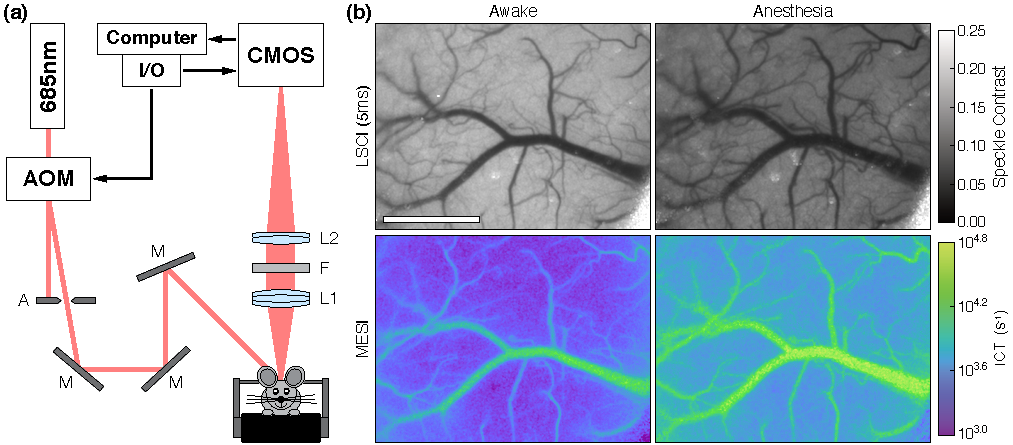
\includegraphics[width=6.25in]{Figure1.pdf}
        \end{tabular}
    \end{center}
    \caption {
        \label{fig:system_image}
        (a) MESI system schematic with 2$\times$ magnification: A (Standard Iris, ID15, Thorlabs, Inc.), M ({{\O}}1$''$ Broadband Dielectric Mirror, BB1-E02, Thorlabs, Inc.), L1 ($f =$ 50 mm, Steinheil Triplet Achromatic, 67-422, Edmund Optics, Inc.), F (685 $\pm$ 20 nm bandpass filter, S685/40m, Chroma Technology Corp.), and L2 ($f = 100$ mm, Achromatic Doublet, AC254-100-A, Thorlabs, Inc.). (b) Single exposure LSCI (5 ms) and MESI inverse correlation time during awake and anesthetized states in Subject 1 (Scale bar = 1 mm) (Video 1, MPEG4, 35.8 MB).
    }
\end{figure}

The temporal dynamics of the awake-to-anesthetized transition can be seen in Fig.~\ref{fig:acute}, where the change in blood flow within two veins (R1 and R2) and one parenchyma region (R3) were analyzed during the extended two-hour imaging session in Subject 1. The cross sections used to estimate $d_{vessel}$ are depicted in Fig.~\ref{fig:acute}a with the resulting changes in vessel diameter shown in Fig.~\ref{fig:acute}b. The width of the two vessels remained steady throughout the awake measurements but increased under anesthesia, with the larger vessel (R1) growing by over 50\% after an hour of exposure. This vasodilation was also accompanied by an increase in blood flow as measured by the relative changes in vascular flux and parenchymal tissue perfusion (Fig.~\ref{fig:acute}c). The vascular flux in R1 and R2 increased by 267\% and 175\%, respectively, while the tissue perfusion in R3 grew by 161\%. The large deviation shortly after $t = 80$ minutes was caused by the subject briefly experiencing breathing difficulties that required the anesthesia to be reduced to 1.5\% isoflurane for several minutes. The breathing abnormality and change in anesthesia dosage had no apparent effects on the vessel size. Repeated measurements in the subject (Figs.~\ref{fig:acute}d-f) illustrate the stability of day-to-day MESI estimates of blood flow as well as the consistency of the hemodynamic response to the isoflurane anesthesia.

% Figure 2 - Extended Awake to Anesthetized Measurements
\begin{figure}
    \begin{center}
        \begin{tabular}{c}
            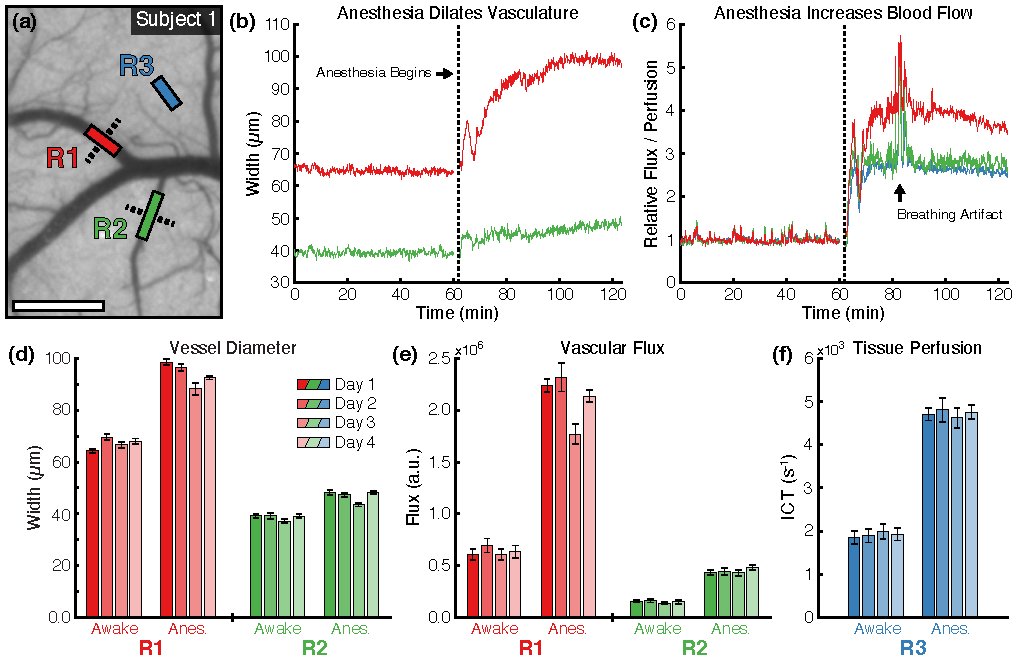
\includegraphics[width=6.25in]{Figure2.pdf}
        \end{tabular}
    \end{center}
    \caption {
        \label{fig:acute}
        (a) Awake speckle contrast image (5 ms) from Subject 1 overlaid with vascular (R1 and R2) and parenchyma (R3) regions used during flow analysis (Scale bar = 500 $\mu$m). Dashed lines indicate the cross-sectional profiles used to calculate vessel width. Timecourses of (b) vessel diameter and (c) relative change in blood flow within the regions over the extended two-hour imaging session. The vertical dashed line indicates the beginning of anesthesia induction. The relative vascular flux and tissue perfusion in (c) were computed using the average of the entire awake state for the baseline. Repeated measurements of (d) vessel diameter, (e) vascular flux, and (f) parenchyma tissue perfusion during awake and anesthetized states in Subject 1 across four imaging sessions (mean $\pm$ sd). Statistics computed across the 50 MESI frames acquired in each state.
    }
\end{figure}

The repeatability of these measurements were further demonstrated across Subjects 2-4 as shown in Fig.~\ref{fig:summary}. Two vascular regions (R1 and R2) and two parenchyma regions (R3 and R4) were examined in each animal during the awake and anesthetized states across three separate imaging sessions lasting 30 minutes each. Similar to the results seen in Fig.~\ref{fig:acute}, the vasodilatory effects of isoflurane anesthesia induced large changes in the cortical hemodynamics. On average, vessel width increased by 13\% and vascular flux increased by over 80\%, with the exception of R2 from Subject 2, which only experienced minimal vasodilation (+1.4\%) and therefore a smaller increase in vascular flux (+63\%). The perfusion of parenchymal regions increased on average by 80\% across all three subjects.

% Figure 3 - Awake to Anesthetized Results Summary
\begin{figure}
    \begin{center}
        \begin{tabular}{c}
            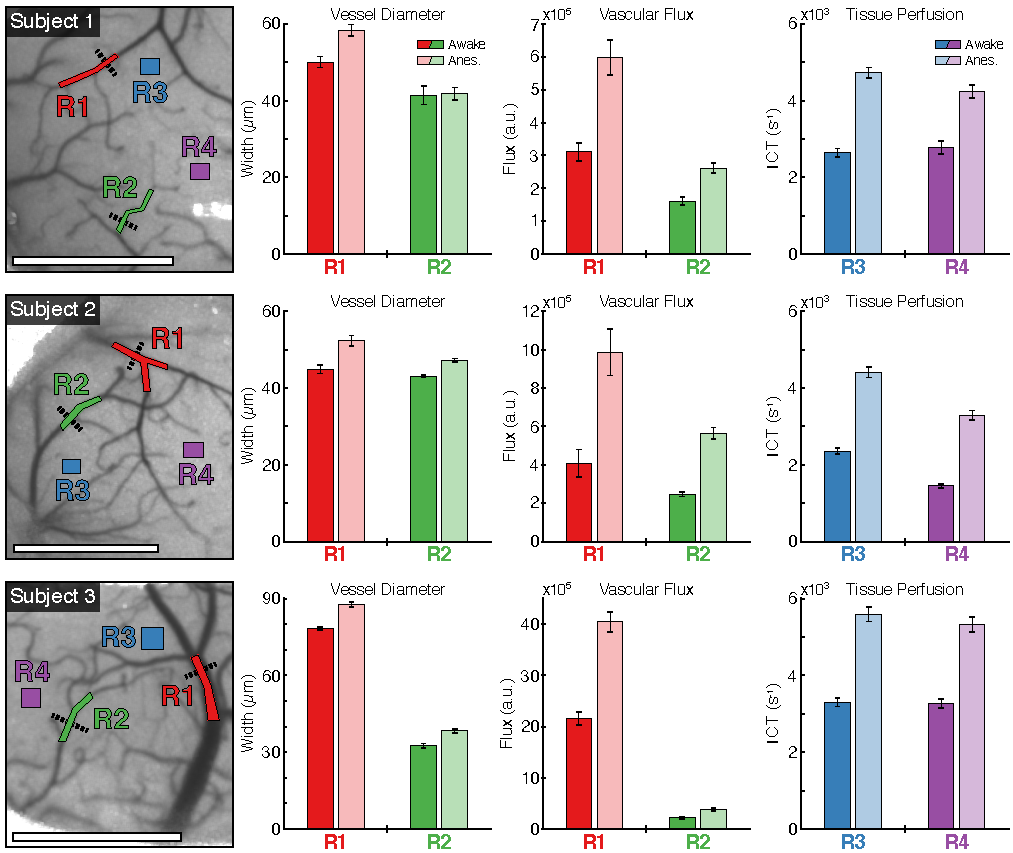
\includegraphics[width=6.25in]{Figure3.pdf}
        \end{tabular}
    \end{center}
    \caption {
        \label{fig:summary}
        Awake speckle contrast images (5 ms) from Subjects 1-3 overlaid with vascular (R1 and R2) and parenchyma (R3 and R4) regions used during flow analysis (Scale bars = 500 $\mu$m). Dashed lines indicate the cross-sectional profiles used to calculate vessel width. Each row of charts depicts vessel diameter, vascular flux, and parenchyma tissue perfusion during awake and anesthetized states averaged across three separate imaging sessions for each subject (mean $\pm$ sd). Statistics computed across each imaging session with uncertainty propagation from the 50 MESI frames acquired in each state.
    }
\end{figure}


% ----------------------------------------------------------------------------------------
% BEGIN DISCUSSION SECTION
% ----------------------------------------------------------------------------------------
\section{Discussion}
\label{sect:discussion}

The systemic effects of isoflurane undermine the reliability of neurophysiological and behavioral studies because anesthesia is a fundamentally unnatural physiological state \cite{Gao:2017tw}. Imaging blood flow on the cortical surface with MESI during the induction of anesthesia directly visualizes and quantifies these large hemodynamic changes. On average, the vasodilation caused by isoflurane increased vessel diameter by 18 $\pm$ 13\% across all trials with large vessel-to-vessel variation but small day-to-day variation (Fig.~\ref{fig:summary}). Direct microscope measurements in fentanyl- and nitrous oxide-anesthetized rats documented a 17\% increase in arteriolar diameter and 6\% increase in venule diameter after the topical application of isoflurane \cite{Koenig:1994rn}. Similar measurements in pentobarbital-anesthetized dogs observed 10-28\% increases in the diameter of small arterioles following the inhalation of isoflurane \cite{Iida:1998th}. Both studies found that isoflurane dilated arterioles in a concentration-dependent manner.

Much larger changes in blood flow were measured in the surface vessels, with vascular flux increasing on average by 135 $\pm$ 64\% across all trials. Even vessels that experienced only minimal vasodilation, such as R2 for Subject 2 in Fig.~\ref{fig:summary}, exhibited an over 60\% increase in flow as measured with MESI. Because few imaging modalities are capable of measuring the dynamics of blood flow with sufficient spatial resolution to distinguish individual vessels, there has been limited work on this topic in awake animals. One study using laser Doppler flowmetry found only non-significant 18\% increases in both CBF and red blood cell (RBC) velocity in the barrel cortex after mice were anesthetized with isoflurane \cite{Takuwa:2012ee}. However, because large blood vessels were avoided, the laser Doppler measurements likely sampled smaller subsurface vasculature that may exhibit different responses to isoflurane than the larger surface vasculature imaged by MESI. The vascular flux metric calculated from the speckle correlation time is also not analogous to either the CBF or RBC velocity measured by laser Doppler flowmetry, so the results are not directly comparable \cite{Kazmi:2015du}.

Within the parenchyma, perfusion increased on average by 92 $\pm$ 35\% across all trials after isoflurane exposure. The reduced variability compared to the vascular measurements is likely a byproduct of the more homogenous structure of the unresolvable capillaries within the parenchyma. fMRI measurements in isoflurane-anesthetized rats have reported $\sim$50\% increases in global CBF with the cerebral cortex experiencing the smallest regional increase (20\%) compared to the awake state \cite{Sicard:2003dj}. However, these numbers are not directly comparable because fMRI samples a much larger volume of the brain than MESI, which has both a smaller field of view and only penetrates several hundred microns into the cortex.

While LSCI has been utilized extensively with awake imaging \cite{Takuwa:2011jr,Seto:2014ga,Lu:2017bo,Balbi:2017cj,Sunil:2020ac}, this is one of the first uses of MESI in an awake animal model \cite{He:2020}. Traditional single-exposure LSCI would likely have underestimated the magnitude of the flow changes caused by isoflurane because individual exposure times are only sensitive to a small range of flow rates \cite{Parthasarathy:2008el}. Failing to account for the increase in multiple dynamic scattering events caused by vasodilation would also have resulted in an underestimation of the flow changes in the visible surface vasculature. Using the raw $ICT$ value instead of the diameter-scaled vascular flux metric in Fig.~\ref{fig:acute}c would have measured only a 140\% increase in the large vessel instead of 267\%. The repeatability of the day-to-day measurements further demonstrate the robustness of MESI as a chronic blood flow imaging technique \cite{Kazmi:2013hp}, even when observing a fully-conscious, moving animal.

The effects of isoflurane fundamentally undermine the imaging of cortical hemodynamics in the normal physiological state. Blood flow imaging techniques such as LSCI, laser Doppler flowmetry, and fMRI require greater sensitivity because of the suppression of the hemodynamic response \cite{Takuwa:2012ee} and measure a delayed neurovascular coupling \cite{Pisauro:2013cx}. Anatomical imaging with two-photon microscopy only captures heavily-dilated vasculature unrepresentative of the awake resting state \cite{Lyons:2016bd}. The consistency and reliability of all imaging techniques can suffer from the effects of prolonged isoflurane exposure, which can cause continual vasodilation as seen in Fig.~\ref{fig:acute}b. This may result in extended imaging sessions documenting disparate anatomies and physiologies between the beginning and conclusion of an experiment.


% ----------------------------------------------------------------------------------------

\subsection{Limitations}

The impact of repeated exposure to isoflurane was not examined in this study. Previous work has found that it can impair synaptic plasticity in the basolateral amygdala \cite{Long:2016ri} and cause persistent motor deficits via structural changes to the corpus callosum \cite{Bajwa:2018ri}. The one day interval between imaging sessions may not have been sufficient to completely avoid these effects despite only 20 minutes of isoflurane exposure. Because the experiment imaged the induction of general anesthesia from the awake state, tracheal intubation for mechanical ventilation was not an option. This may result in breathing variability that impacts the systemic hemodynamics and complicates comparisons with other studies that had mechanical control of ventilation. Since varying the isoflurane dosage was the only method of regulating breathing stability, the concentration dependent effects of isoflurane may have also influenced the results \cite{Masamoto:2009dd,Li:2014eh}.

While image registration can help maintain the spatial alignment of data across an experiment, it is unable to decouple the effects of animal motion from the underlying blood flow. Even with the head fully restrained, walking and grooming both cause subtle brain movements that manifest as large changes in speckle contrast, as seen by the abrupt spikes during the awake section of Fig.~\ref{fig:acute}c. While these fluctuations may characterize real hemodynamic responses, it is difficult to isolate them from broader animal motion. A simple solution might be the addition of an external sensor to the treadmill \cite{Dombeck:2007gr} to exclude timepoints when the animal is actively moving. However, a more refined awake imaging system that further minimizes brain movement would likely be necessary to directly probe these phenomena with LSCI or MESI.


% ----------------------------------------------------------------------------------------
% BEGIN CONCLUSION SECTION
% ----------------------------------------------------------------------------------------
\section{Conclusion}
\label{sect:conclusion}

We have used MESI to image CBF during the induction of general anesthesia with isoflurane in head-restrained mice. The vasodilatory effects of isoflurane caused large anatomical and physiological changes that were drastically different from the awake state. These increases in vessel size and blood flow were repeatable across multiple imaging sessions in the same subjects. This study also demonstrated that the MESI technique can be readily used for chronic awake imaging and allows for direct day-to-day comparisons of blood flow. These results provide further evidence that the anesthetized state is unrepresentative of normal physiology and that neurophysiological and behavioral experiments would benefit immensely from transitioning to un-anesthetized awake animal models.


% ----------------------------------------------------------------------------------------
% BEGIN DISCLOSURES AND ACKNOWLEDGEMENTS
% ----------------------------------------------------------------------------------------
\subsection*{Disclosures}
A.K.D. holds equity in Dynamic Light, Inc. The authors declare no other conflicts of interest.

\subsection*{Author Contributions}
C.T.S. and L.M.R. constructed the imaging system, conceived the experiments, and acquired the data. C.T.S analyzed the results and wrote the manuscript. F.H. performed the animal surgeries. L.L. and A.K.D. supervised the project. All authors contributed to the manuscript revisions.

\acknowledgments
This study was supported by the National Institutes of Health (Nos. EB011556, HL140153, NS108484, NS109361, and T32EB007507).


% ----------------------------------------------------------------------------------------
% BEGIN BIBLIOGRAPHY
% ----------------------------------------------------------------------------------------
\bibliography{bibliography.bib}
\bibliographystyle{spiejour} % SPIE bibliography style


% ----------------------------------------------------------------------------------------
% AUTHOR BIOGRAPHIES
% ----------------------------------------------------------------------------------------
\vspace{1ex}
\vspace{2ex}\noindent\textbf{Colin T. Sullender} received his PhD in biomedical engineering from the University of Texas at Austin in 2018. Currently, he is a postdoctoral research fellow working with Dr. Andrew Dunn in the Functional Optical Imaging Laboratory (FOIL) at the University of Texas. His research focuses on the continued development and clinical translation of the laser speckle contrast imaging technique.

\vspace{2ex}\noindent\textbf{Lisa M. Richards} received her PhD in biomedical engineering from the University of Texas at Austin in 2015. Currently, she is a Senior Biomedical Systems Engineer at Seno Medical Instruments.

\vspace{2ex}\noindent\textbf{Fei He} received his PhD in optical engineering from the Chinese Academy of Sciences. Currently, he is a postdoctoral research fellow working with Dr. Lan Luan in the Luan Laboratory of Integrative Neural Interface at Rice University.

\vspace{2ex}\noindent\textbf{Lan Luan} is an Assistant Professor in the Department of Electrical and Computer Engineering at Rice University and a member of the Rice Neuroengineering Initiative. Her research focuses on the development of multimodal neural interfaces that combine electrical, optical, and other technologies to monitor and manipulate brain activity.

\vspace{2ex}\noindent\textbf{Andrew K. Dunn} is the Donald J. Douglass Centennial Professor of Engineering in the Department of Biomedical Engineering at the University of Texas at Austin and the Director of the Center for Emerging Imaging Technologies. His research focuses on the development of innovative optical imaging techniques for studying the brain.


% ----------------------------------------------------------------------------------------
% FIGURE AND TABLE LISTS
% ----------------------------------------------------------------------------------------
\listoffigures

\end{spacing}
\end{document}

% ----------------------------------------------------------------------------------------
% END
% ----------------------------------------------------------------------------------------